\documentclass{article}
\usepackage{graphicx}
\usepackage{caption}
\usepackage{subcaption}
\usepackage{amssymb}
\usepackage{amsmath}
\usepackage{float}

\usepackage[margin=1in]{geometry}


\begin{document}



\title{16-720 Computer Vision: Homework 5}
\author{Xiang Zhi Tan}

\maketitle
\subsection*{Q1.0}
$(M - w) \times (N - h)$ windows

\subsection*{Q1.2}
In cases where the positive data is rare like 99\% negative and 1\% positive data. A classifier could always return negative and still have a 99\% accuracy and it is actually doing pretty bad. However, the precision/recall metric will not have that issue as it will return a lower value for this fake classifier compare to another classifier that might have only an accuracy of 90\% but tries to classifies the data correctly.

\subsection*{Q1.3}
1000 Exemplar detectors, and one Dalal-Triggs type detector.


\subsection*{Q2.1}
A lower bandwidth will cause more clusters to form as it will find the different local maxima density in each clusters. I ended up using the bandwidth of $35$ through observation of the resulting figure as the bandwidth should be the radius for the clustering circle we want to form. Following is the figure showing the result of the mean shift algorithm with the bandwidth of $35$:
\begin{figure}[H]
    \centering
    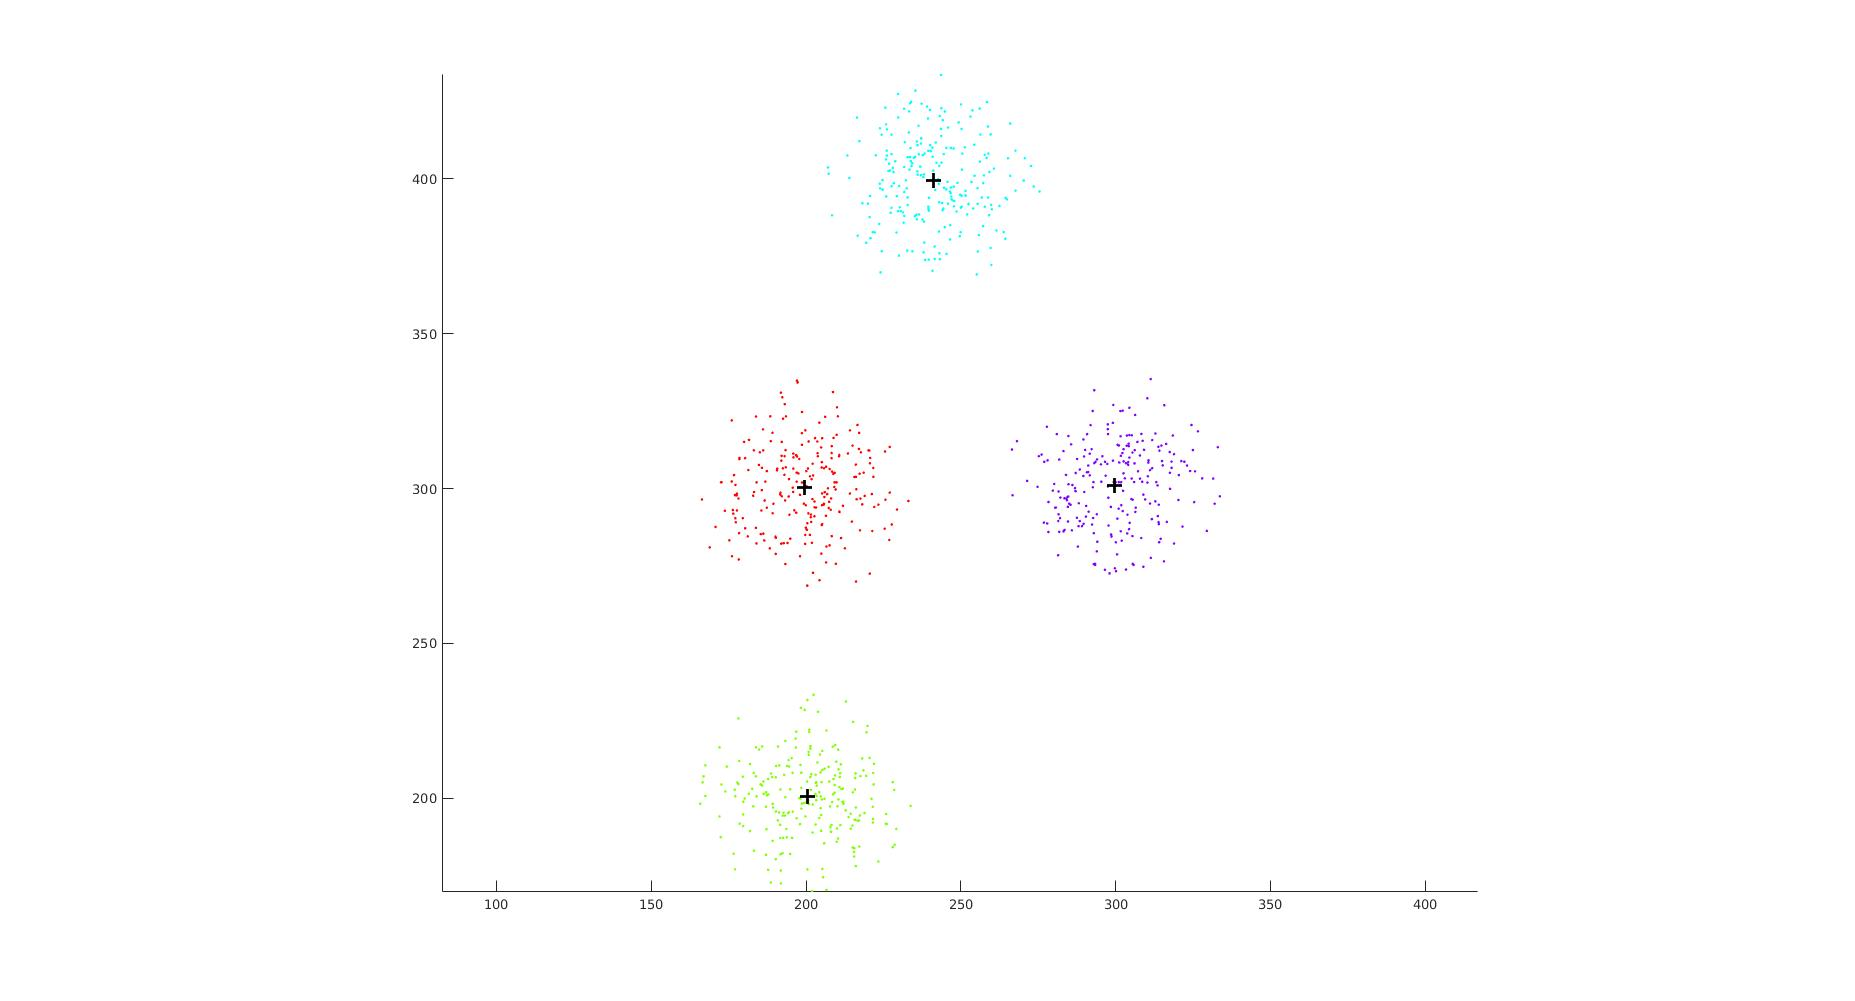
\includegraphics[width=6.5in]{./figures/q21_35.jpg}
    \caption{Grouping of points with bandwidth of $35$}
\end{figure}

\subsection*{Q2.2.2}
When there is more than K number of clusters, I selected the best clusters based on the numbers of memberships in the clusters. My rational is that the best centers would have more members than others, therefore the clusters with the most members are selected and if there are ties, one of them are randomly selected. Following are the images provided and I found online that shows the NMS function.
\begin{figure}[H]
    \centering
    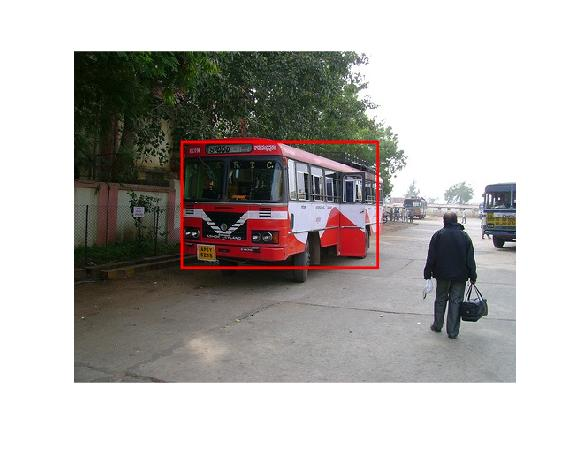
\includegraphics[width=3in]{./figures/q42_result0.jpg}
    \caption{correctly identify bus from test image}
\end{figure}
\begin{figure}[H]
    \centering
    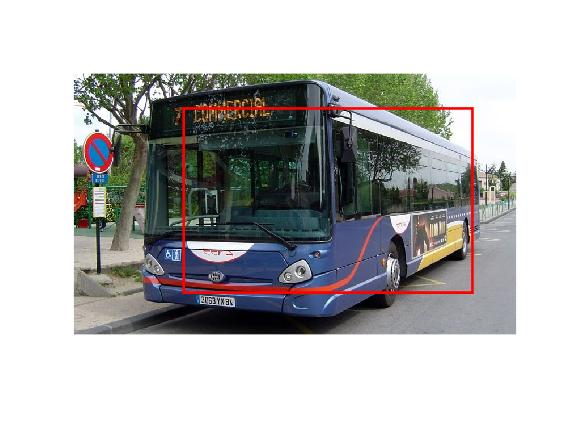
\includegraphics[width=3in]{./figures/q42_result1.jpg}
    \caption{correctly identify bus from google searched image}
\end{figure}
\begin{figure}[H]
    \centering
    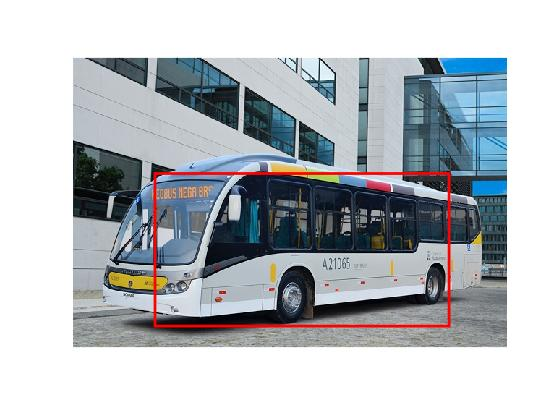
\includegraphics[width=3in]{./figures/q42_result2.jpg}
    \caption{correctly identify bus from google searched image}
\end{figure}
\begin{figure}[H]
    \centering
    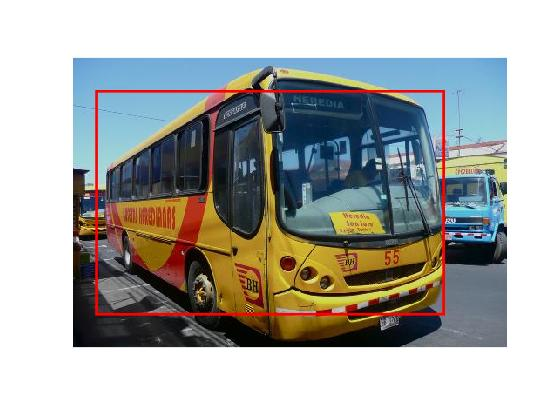
\includegraphics[width=3in]{./figures/q42_result3.jpg}
    \caption{correctly identify bus from google searched image}
\end{figure}

\subsection*{Q3.1}
Average Precision calculates the area under the Precision/Recall curves. This means that Average Precision is higher for classifiers that has less false positive at lower recalls than those that don't.

\subsection*{Q3.2}
\begin{figure}[H]
    \centering
    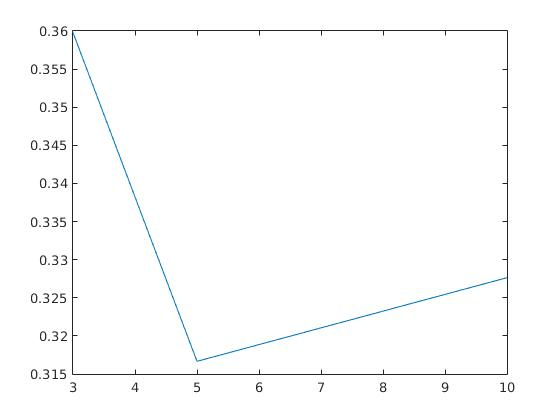
\includegraphics[width=6.5in]{./figures/q33.jpg}
    \caption{Average Precision against Level per octave}
\end{figure}
From the graph, we observe that having more levels per octave would give us a lower Average Precision which means that the higher the level, the more false positive there is.

\subsection*{Q3.3}
Following is the number of k detectors against the AP.
\begin{figure}[H]
    \centering
    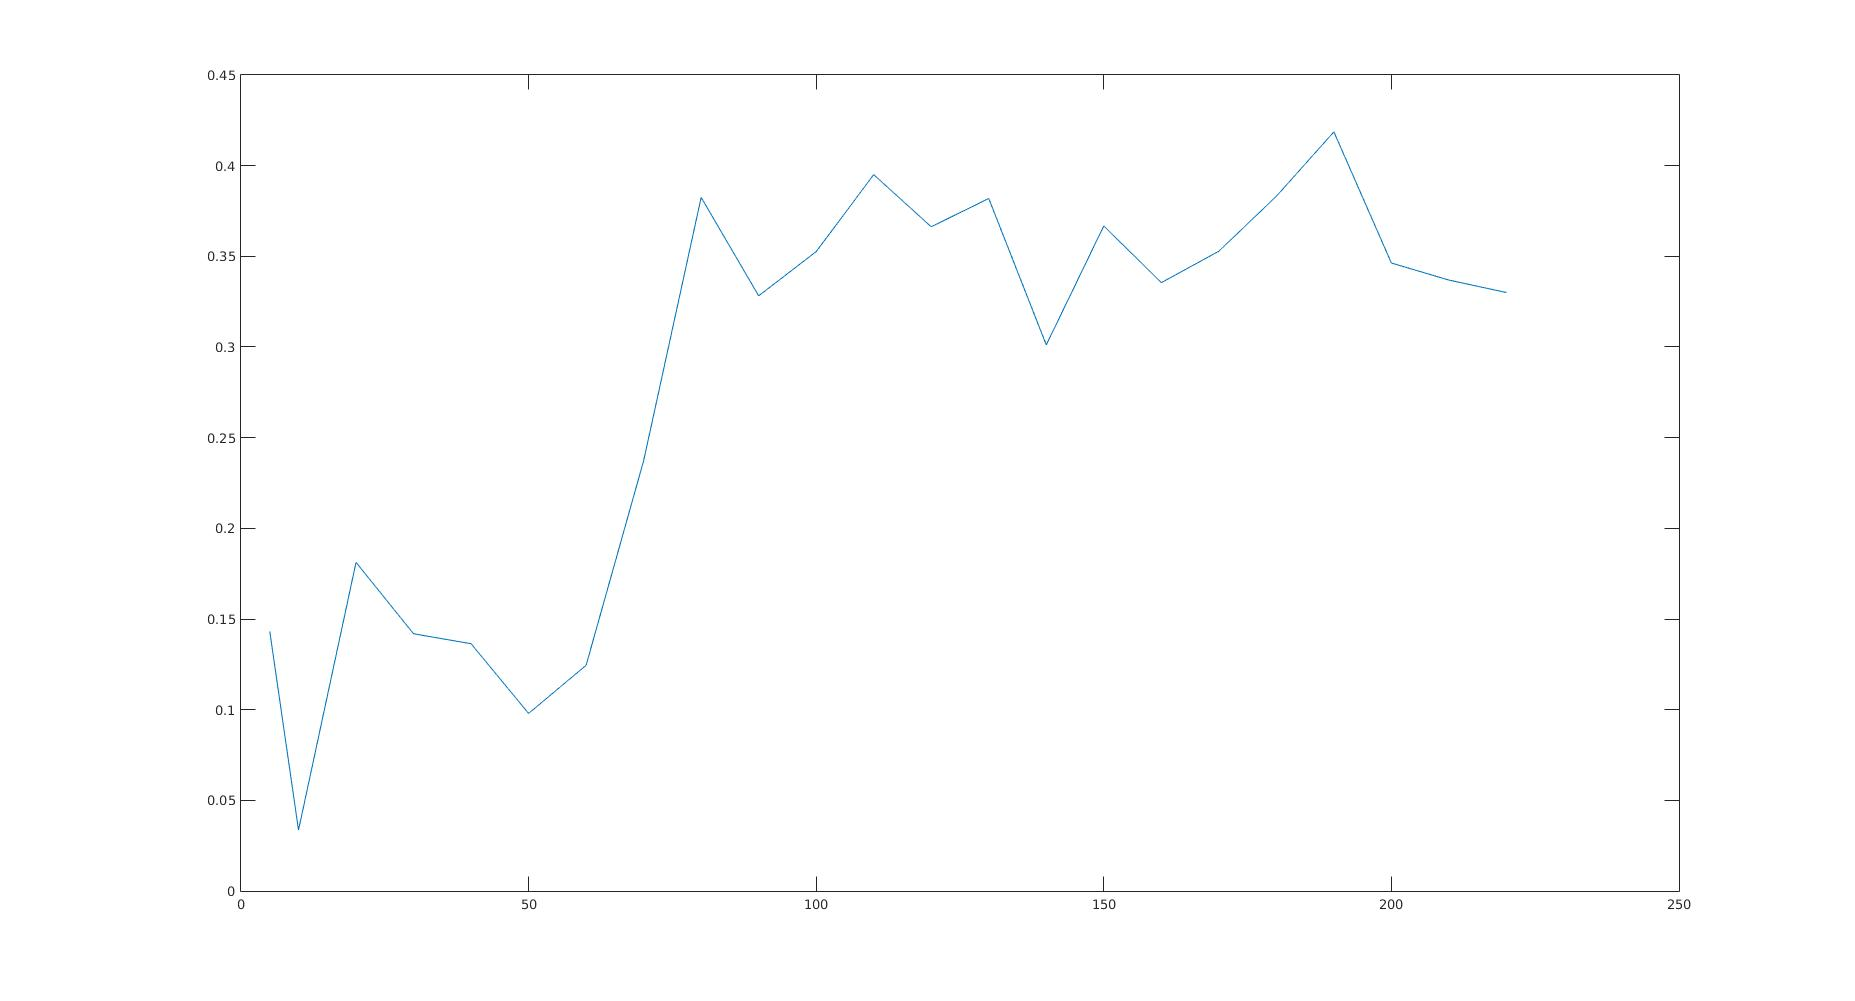
\includegraphics[width=6.5in]{./figures/q34_plot.jpg}
    \caption{Average Precision against number of K}
\end{figure}
From the graph we can see that the performance plateaued after reaching around $k=80$. The fluctuation in the result is caused by the K-mean initialization and has a large variation between each runs. From the graph, one of the highest AP for the feature is around $0.395057$ with $k=110$. Using $k=110$, I generated the following average image:
\begin{figure}[H]
    \centering
    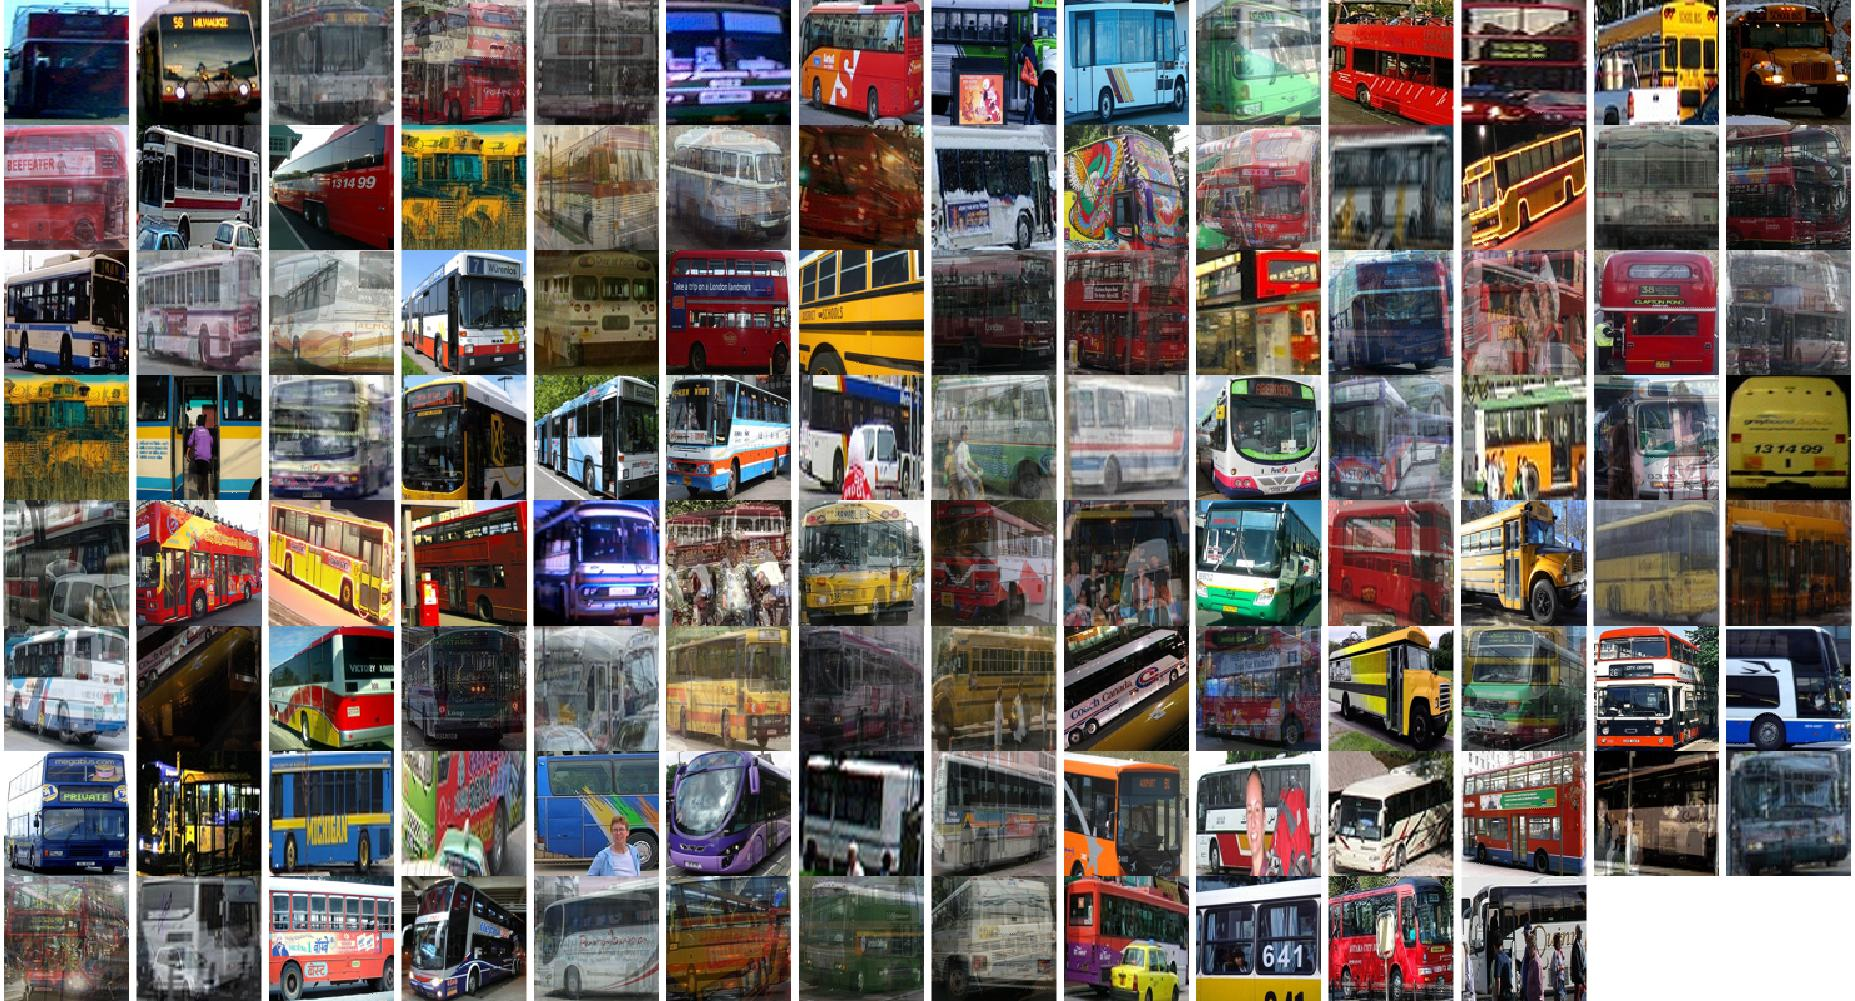
\includegraphics[width=6.5in]{./figures/q34_graph.jpg}
    \caption{Filter Bank features with $k=110$}
\end{figure}
\subsection*{Q3.4}
I used the BRIEF feature descriptor that we used back in HW2 as my feature. I modified it such that it makes $512$ uniformly distributed pair-wise comparison over the whole $100 \times 100$ image after the resize. Following is the number of k detectors against the AP.
\begin{figure}[H]
    \centering
    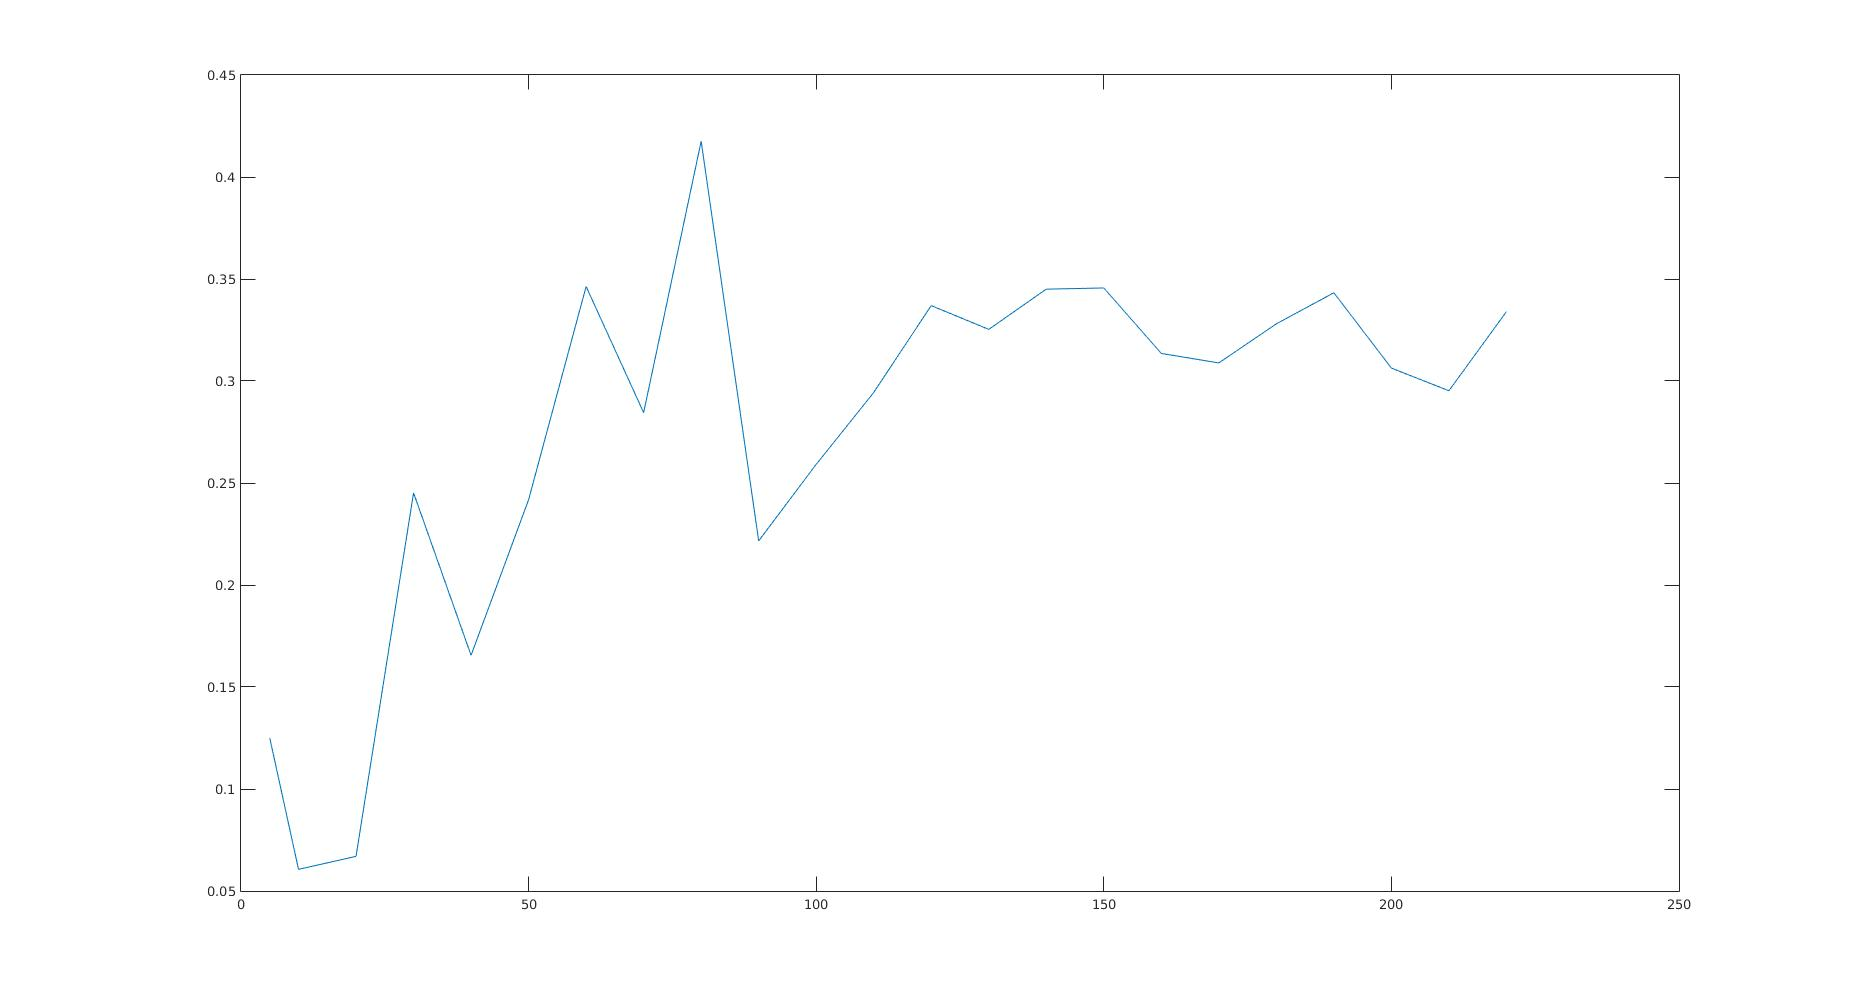
\includegraphics[width=6.5in]{./figures/q35_plot.jpg}
    \caption{Average Precision against number of K}
\end{figure}
The highest AP for the feature is around $0.417553$ with $k=80$. Using $k=80$, I generated the following average image:
\begin{figure}[H]
    \centering
    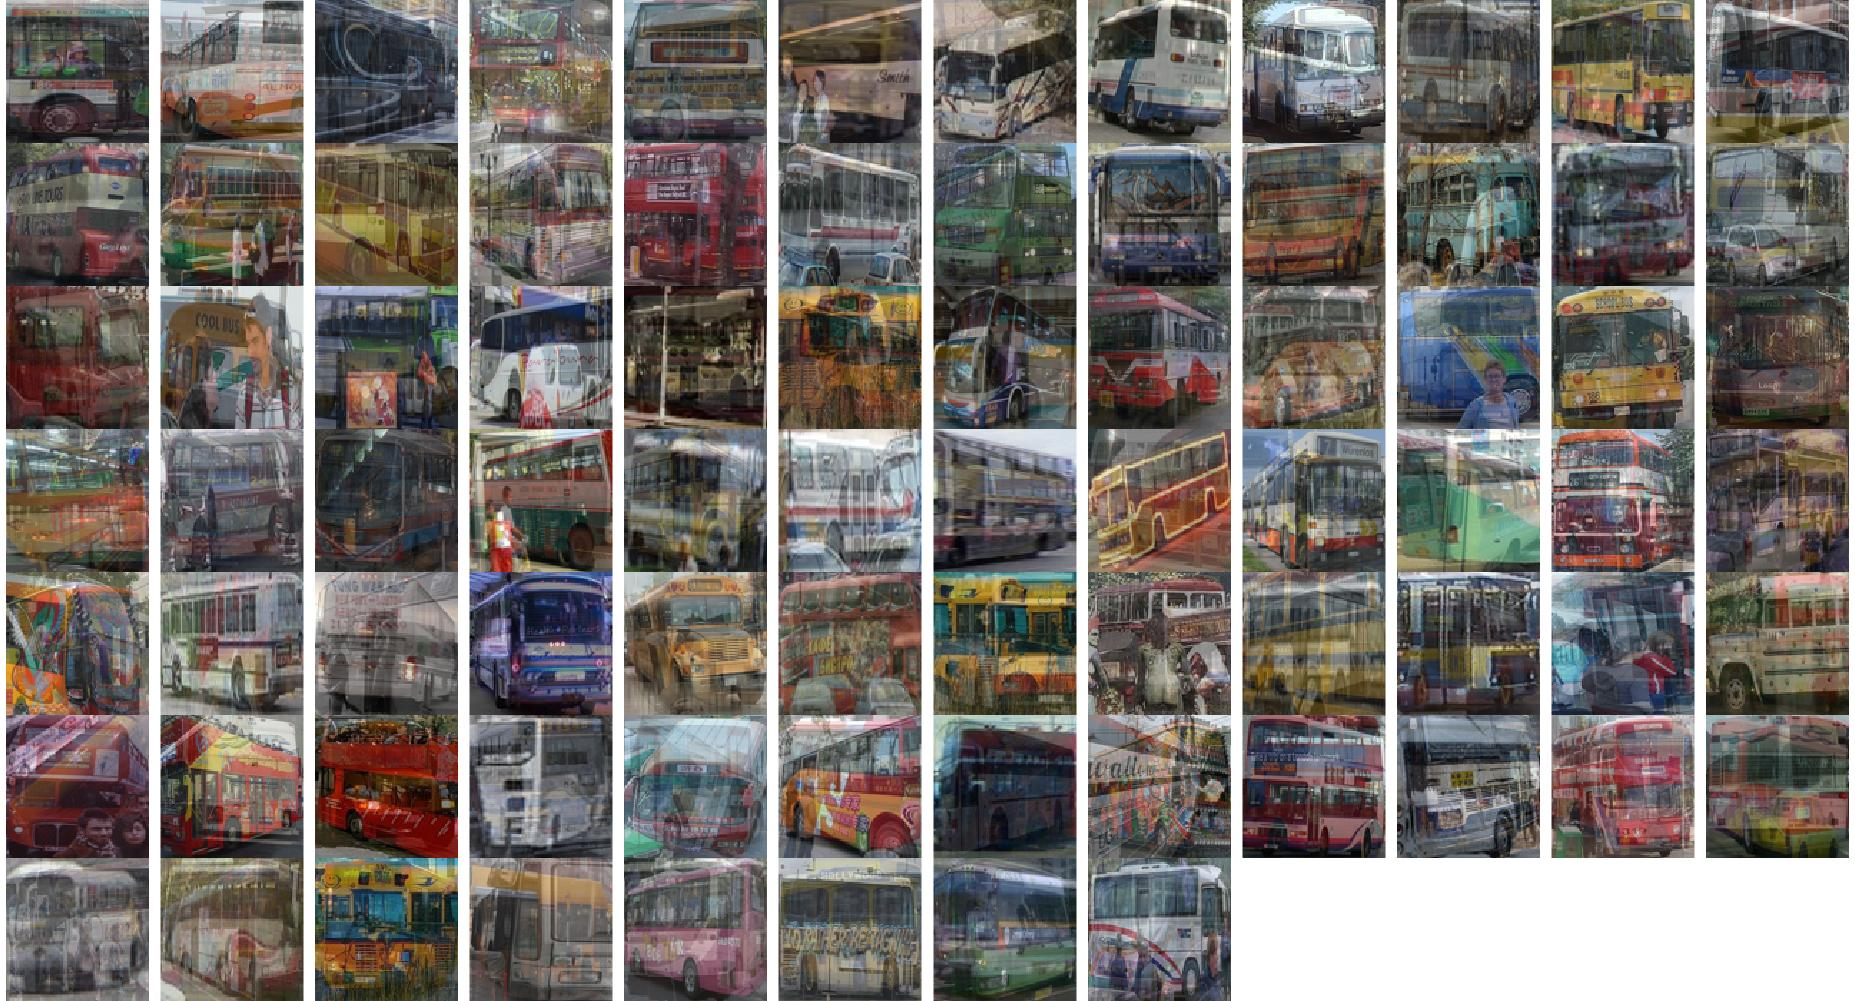
\includegraphics[width=6.5in]{./figures/q35_graph.jpg}
    \caption{512 bits BRIEF features with $k=80$}
\end{figure}
\end{document}